% !TeX encoding = UTF-8
% !TeX spellcheck = sk_SK
% !TeX root=teoriaprocesovtakac.tex
\section{Kyslíkový konvertor}

Kyslíkový konvertor
\begin{enumerate}
\item{čo to je (o aký technologický proces sa jedná, vstupy, výstupy ...)}
\item{rozdelenie na elementárne procesy}
\item{stručne popísať jednotlivé elementárne procesy}
\end{enumerate}

V oceliarstve nastal počas druhej polovice 20. storočia významný posun a progres vo vývoji technológií a procesov výroby ocele. Jedným z najdôležitejších milníkom bolo prvé spustenie komerčnej prevádzky výroby ocele vháňaním kyslíka do konvertora začiatkom 50. rokov minulého storočia v mestách Linz (firma VÖEST) a Donawitz (forma ÖAMG) v Rakúsku. Z názvov týchto miest pochádza aj pomenovanie spôsobu výroby ocele praktizovanom v kyslíkových konvertoroch, a to LD proces, a zároveň aj názov samotného kyslíkového konvertora (LD konvertor). Postupom času a zdokonaľovaním LD procesu sa LD konvertory rozšírili do celého sveta a už niekoľko rokov sú najvyužívanejšou technológiou pre výrobu ocele na celom svete.

\begin{figure}
\centering
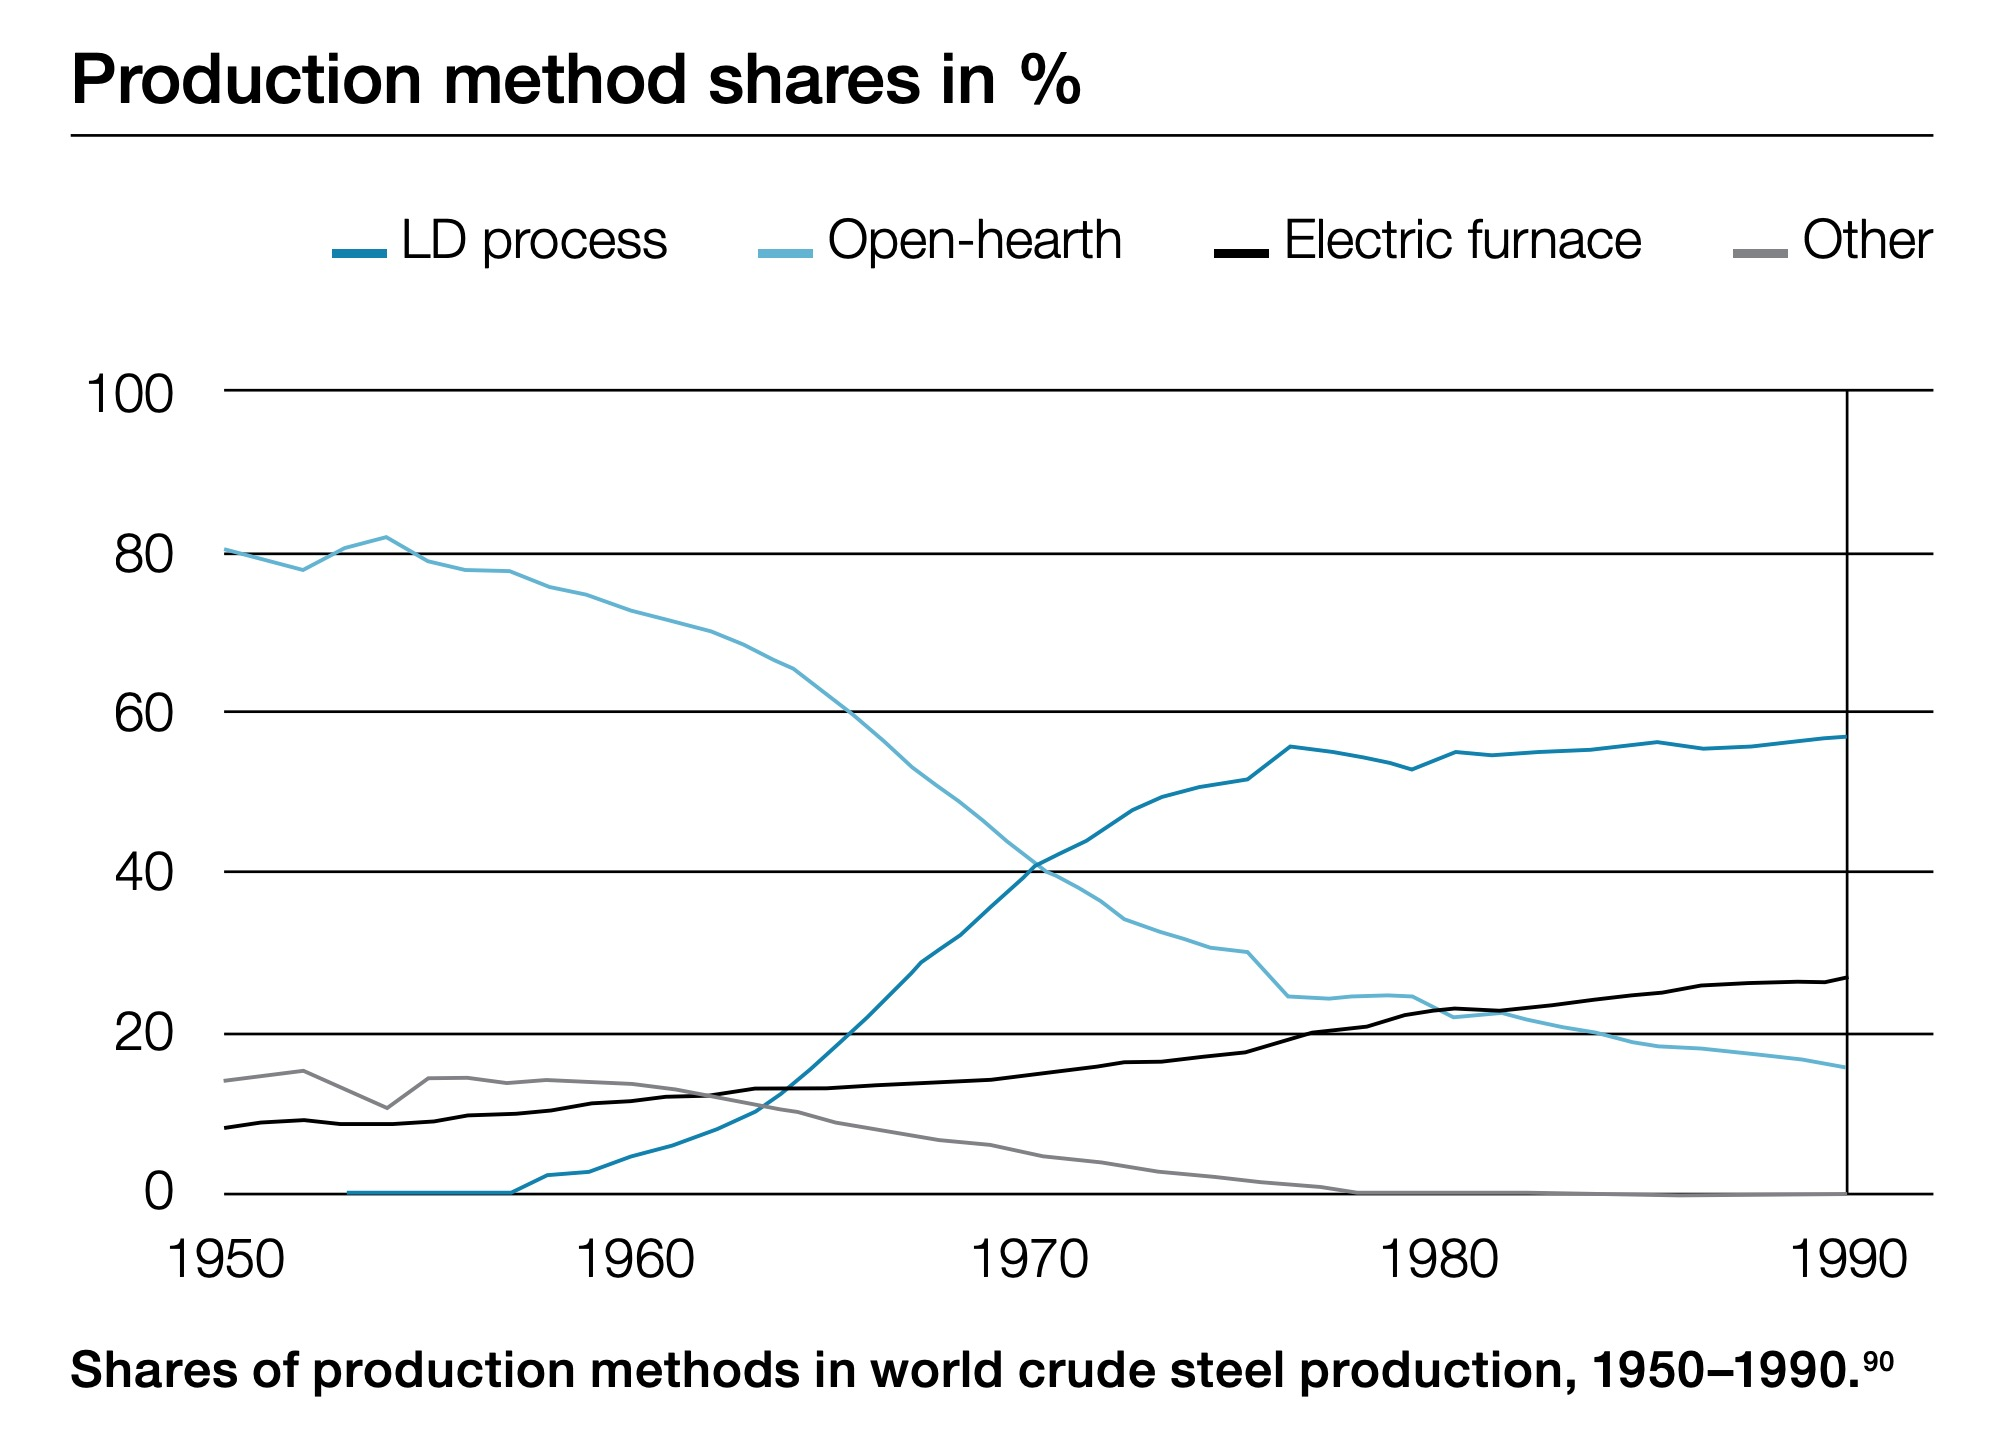
\includegraphics[width=.9\textwidth,angle=0]{ld-process-history-data.jpg}
\caption{Podiel výrobných medód ocele v percentách \citep{voestalpineLD2012}}
\label{o:1}
\end{figure}

Spomínaný LD proces sa v rôznych častiach sveta názýva odlišne. Napríklad vo Veľkej Británii sa označuje ako BOS (basic oxygen steelmaking); v Amerike a v Ázijských krajinách BOF (basix oxygen furnace) s výnimkou americkej korporácie U.S. Steel, kde sa často označuje ako BOP (basic oxygen process) \citep{Turkdogan1996}.

\begin{figure}
\centering
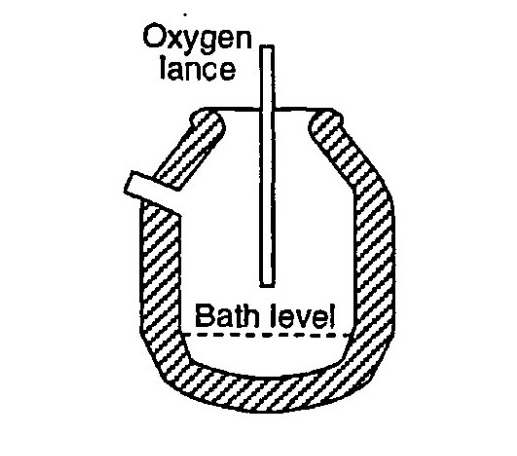
\includegraphics[width=.5\textwidth,angle=0]{bof-single.jpg}
\caption{Výroba ocele v konvertore fúkaním kyslíka zhora \citep{Turkdogan1996}.}
\label{o:2}
\end{figure}

V 70. rokoch bol v Kanade a Nemecku vyvinutý (a následne komercializovaný) upravený typ konvertora s vháňaním kyslíka z dolnej časti. Tento proces sa v Európe označuje ako OBM a v iných častiach sveta ako Q-BOP.

\begin{figure}
\centering
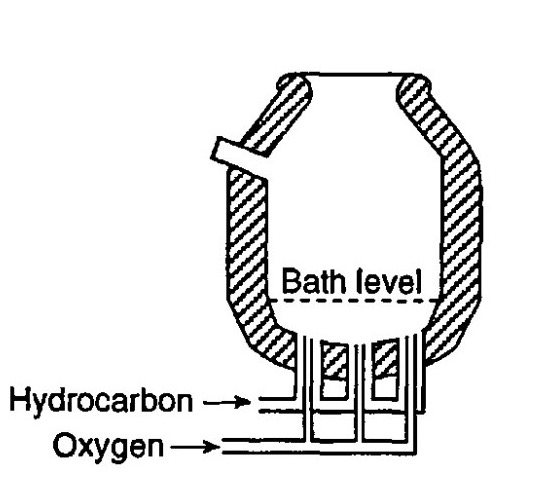
\includegraphics[width=.5\textwidth,angle=0]{q-bop.jpg}
\caption{Výroba ocele v konvertore fúkaním kyslíka zdola \citep{Turkdogan1996}.}
\label{o:3}
\end{figure}

V konvertore pre Q-BOP proces sa v dolnej časti nachádzajú trysky vsadené do odnímateľného dna, cez ktoré sú vháňané kyslík (\ce{O2}) spolu s páleným vápnom a prstencová medzera okolo centrálnej rúry na priechod plynného uhľovodíka (napr. propán alebo metán). Po kontakte s tekutou oceľou uhľovodík disociuje na \ce{C} a \ce{H2} pri absorpcii tepla. Táto endotermická reakcia potláča prehrievanie hrotu vyhadzovača exotermickou reakciou kyslíka s tekutou oceľou.

Ďalší vývojovým krokom výroby ocele v kyslíkovom konvertore bolo spojenie typov fúkania kyslíka zhora a zdola.


\begin{figure}[!tbp]
	\centering
	\subfloat[Kombinovaný BOF.]{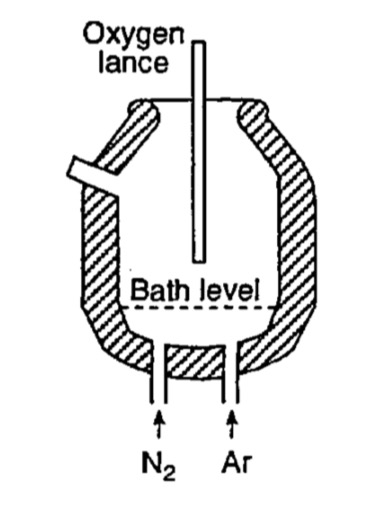
\includegraphics[width=0.38\textwidth]{kombinovany-bof.jpg}\label{fig:f1}}
	\hfill
	\subfloat[Kombinovaný Q-BOP.]{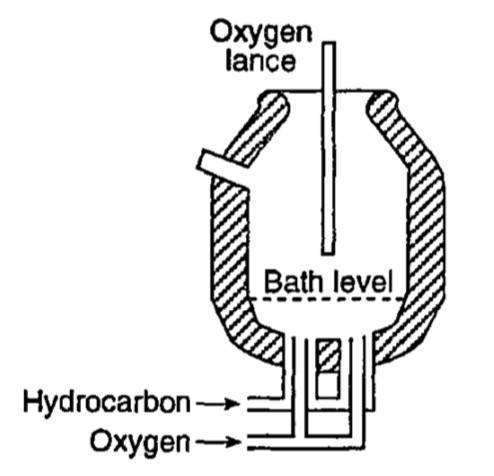
\includegraphics[width=0.52\textwidth]{kombinovany-q-bop.jpg}\label{fig:f2}}
	\caption{Výroba ocele procesom BOF a Q-BOP v LD konvertore s kombinovaným typom fúkania.}
	\label{o:4}
\end{figure}


-----------

Basic oxygen furnace (BOF) steelmaking is a complex process and dynamic model is very important for endpoint control. It is usually difficult to build a precise BOF endpoint dynamic model because many input variables affect the endpoint carbon content and temperature.


BOF is a widely preferred and effective steelmaking method
due to its high productivity and considerably low production cost. Therefore, almost 65\% of the total crude steel productions in the world are melted by using the BOF method. BOF steelmaking is a very complex chemical physical process. The quality of scrap iron changes from batch to batch. The grades of steel produced vary frequently, and the components of raw materials fluctuate largely \cite{Wang2010}.

The main objective of controlling oxygen converter steelmaking is to obtain prescribed parameters for the steel when it is tapped from the furnace, including weight, temperature, and each element content. In practical steelmaking process, the criterion whether the molten steel is acceptable or not is often decided by the endpoint carbon content and temperature.

-----------------------

Pri tejto metóde musí byť ale ešte dodávaná tavenina, aby dávka nevychladla.
Hotová oceľ sa potom vyleje z konvertora do panvy na ďalšie spracovanie.
Cenovo skoro najvýhodnejší spôsob výroby ocele pre veľké množstvá.
